\documentclass[
    language=english,
    doctype=meta-analysis,
    institution=none,
]{../../omnilatex}

\RequirePackage{config/document-settings}

\begin{document}
\maketitle

\begin{abstract}
\textbf{Objective:} To systematically evaluate the efficacy of cognitive behavioral therapy
(CBT) for insomnia (CBT-I) in adults aged 60 and older through a meta-analysis of
randomized controlled trials (RCTs).

\textbf{Methods:} We conducted a systematic search of PubMed, PsycINFO, and Cochrane
CENTRAL from inception through December 2024. We included RCTs comparing CBT-I to
waitlist, attention, or active control conditions in adults $\geq$ 60 years with
diagnosed insomnia. Primary outcomes were sleep onset latency (SOL), wake after sleep
onset (WASO), total sleep time (TST), and sleep efficiency (SE). We used random-effects
models to compute pooled effect sizes (Hedges' $g$).

\textbf{Results:} Of 1,847 identified records, 34 RCTs (total $N = 3,218$) met inclusion
criteria. CBT-I demonstrated significant improvements compared to controls in SOL
($g = -0.68$, 95\% CI $[-0.82, -0.54]$), WASO ($g = -0.59$, 95\% CI $[-0.73, -0.45]$),
TST ($g = 0.47$, 95\% CI $[0.34, 0.60]$), and SE ($g = 0.72$, 95\% CI $[0.58, 0.86]$).
Moderator analyses indicated that delivery format (group vs.\ individual) and treatment
duration moderated efficacy.

\textbf{Conclusions:} CBT-I is an effective treatment for insomnia in older adults, with
moderate-to-large effect sizes across multiple sleep outcomes. Adaptations for this
population, including group delivery and extended treatment duration, may enhance outcomes.
\end{abstract}

\section{Introduction}
\label{sec:introduction}

Insomnia disorder affects approximately 30--50\% of older adults and is associated with
increased risk of cognitive decline, depression, falls, and mortality \cite{morin2011insomnia}.
Cognitive behavioral therapy for insomnia (CBT-I) is recommended as the first-line treatment
by major clinical guidelines, including those of the American College of Physicians
\cite{qaseem2016management}. However, the evidence base for CBT-I specifically in older
adults has not been comprehensively synthesized.

Prior meta-angeles have examined CBT-I efficacy across the lifespan but have not focused
specifically on adults aged 60 and older \cite{trauer2015cognitive}. Given the unique
sleep architecture changes and comorbidity profiles in older adults, a focused meta-analysis
is warranted.

\section{Methods}
\label{sec:methods}

\subsection{Search Strategy}

We developed a comprehensive search strategy in consultation with a medical librarian.
The search combined terms for ``cognitive behavioral therapy,'' ``insomnia,'' ``sleep,''
and ``aged'' with appropriate MeSH headings and free-text synonyms. The full search string
is provided in Appendix~A.

\subsection{Eligibility Criteria}

Studies were included if they met the following PICOS criteria:
\begin{itemize}
    \item \textbf{Population:} Adults aged $\geq$ 60 years with a diagnosis of insomnia
          (clinical or subthreshold).
    \item \textbf{Intervention:} CBT-I, delivered in any format (individual, group, digital).
    \item \textbf{Comparators:} Waitlist, attention control, sleep hygiene education, or
          pharmacotherapy.
    \item \textbf{Outcomes:} At least one objective or subjective sleep measure (SOL, WASO,
          TST, SE, or sleep diary measures).
    \item \textbf{Study Design:} Randomized controlled trials.
\end{itemize}

\subsection{Data Extraction}

Two reviewers independently extracted data on study characteristics, participant demographics,
intervention details, and outcomes. Discrepancies were resolved by consensus or consultation
with a third reviewer. We used a standardized data extraction form in Covidence.

\subsection{Statistical Analysis}

We computed Hedges' $g$ as the effect size metric, which provides a bias-corrected
standardized mean difference. We used random-effects models (restricted maximum likelihood
estimation) to pool effect sizes across studies. Heterogeneity was assessed using $I^2$,
$\tau^2$, and Cochran's $Q$ statistic.

\begin{equation}
    \label{eq:effect-size}
    g = \frac{\bar{X}_1 - \bar{X}_2}{S_{\text{pooled}}} \left(1 - \frac{3}{4(n_1 + n_2 - 2) - 1}\right)
\end{equation}

We conducted moderator analyses using mixed-effects models with the following a priori
moderators: delivery format (individual vs.\ group), treatment duration ($<$ 6 weeks vs.\
$\geq$ 6 weeks), inclusion of sleep restriction therapy, and control condition type.
Publication bias was assessed using funnel plots, Egger's test, and trim-and-fill analysis.

\section{Results}
\label{sec:results}

\subsection{Study Selection}

\begin{figure}[htbp]
    \centering
    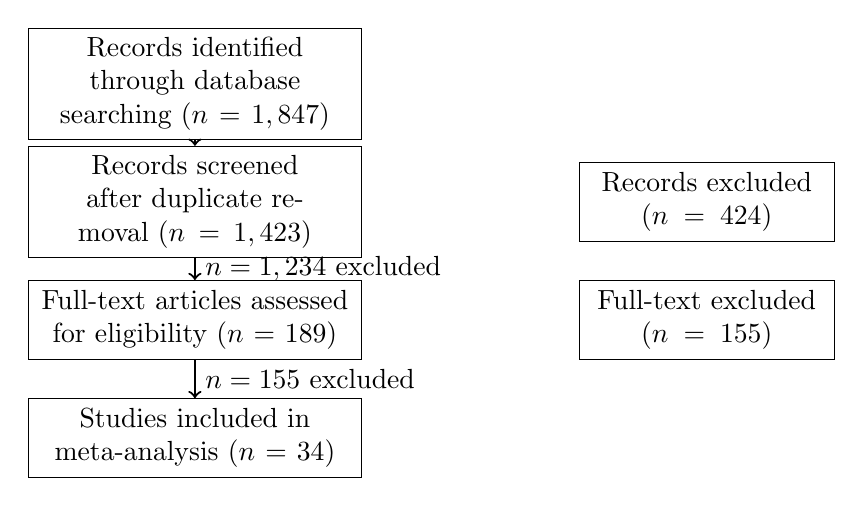
\begin{tikzpicture}[
        node distance=1.5cm,
        box/.style={rectangle, draw, text width=4cm, align=center, minimum height=1cm},
        arrow/.style={->, thick}
    ]
        \node[box] (identified) {Records identified through database searching ($n = 1,847$)};
        \node[box, below of=identified] (screened) {Records screened after duplicate removal ($n = 1,423$)};
        \node[box, below of=screened] (eligible) {Full-text articles assessed for eligibility ($n = 189$)};
        \node[box, below of=eligible] (included) {Studies included in meta-analysis ($n = 34$)};

        \draw[arrow] (identified) -- (screened);
        \draw[arrow] (screened) -- node[right] {$n = 1,234$ excluded} (eligible);
        \draw[arrow] (eligible) -- node[right] {$n = 155$ excluded} (included);

        \node[box, right of=screened, xshift=5cm, text width=3cm] (excluded1) {Records excluded ($n = 424$)};
        \node[box, right of=eligible, xshift=5cm, text width=3cm] (excluded2) {Full-text excluded ($n = 155$)};
    \end{tikzpicture}
    \caption{PRISMA flow diagram of study selection.}
    \label{fig:prisma}
\end{figure}

\subsection{Study Characteristics}

The 34 included RCTs were published between 2005 and 2024. The total sample size was
3,218 participants (mean age range: 62--78 years; range of female proportion: 42--78\%).
Fifteen studies used individual CBT-I delivery, 14 used group delivery, and 5 used digital
delivery. Treatment duration ranged from 2 to 12 weeks (median: 6 weeks).

\begin{table}[htbp]
    \centering
    \caption{Summary of included study characteristics.}
    \label{tab:study-characteristics}
    \begin{tabular}{@{}lc@{}}
        \toprule
        Characteristic & $k$ (studies) \\
        \midrule
        \textbf{Delivery format} & \\
        \quad Individual & 15 \\
        \quad Group & 14 \\
        \quad Digital & 5 \\[6pt]
        \textbf{Treatment duration} & \\
        \quad $<$ 6 weeks & 12 \\
        \quad $\geq$ 6 weeks & 22 \\[6pt]
        \textbf{Control condition} & \\
        \quad Waitlist & 18 \\
        \quad Attention & 10 \\
        \quad Active (sleep hygiene) & 6 \\
        \bottomrule
    \end{tabular}
\end{table}

\subsection{Primary Outcomes}

\begin{table}[htbp]
    \centering
    \caption{Pooled effect sizes for primary sleep outcomes.}
    \label{tab:primary-outcomes}
    \begin{tabular}{@{}lcccccc@{}}
        \toprule
        Outcome & $k$ & $N$ & Hedges' $g$ & 95\% CI & $I^2$ & $p$ \\
        \midrule
        SOL (min) & 28 & 2,640 & $-0.68$ & $[-0.82, -0.54]$ & 68\% & $< .001$ \\
        WASO (min) & 24 & 2,189 & $-0.59$ & $[-0.73, -0.45]$ & 72\% & $< .001$ \\
        TST (min) & 22 & 2,045 & $0.47$ & $[0.34, 0.60]$ & 58\% & $< .001$ \\
        SE (\%) & 30 & 2,876 & $0.72$ & $[0.58, 0.86]$ & 64\% & $< .001$ \\
        \bottomrule
    \end{tabular}
\end{table}

\begin{figure}[htbp]
    \centering
    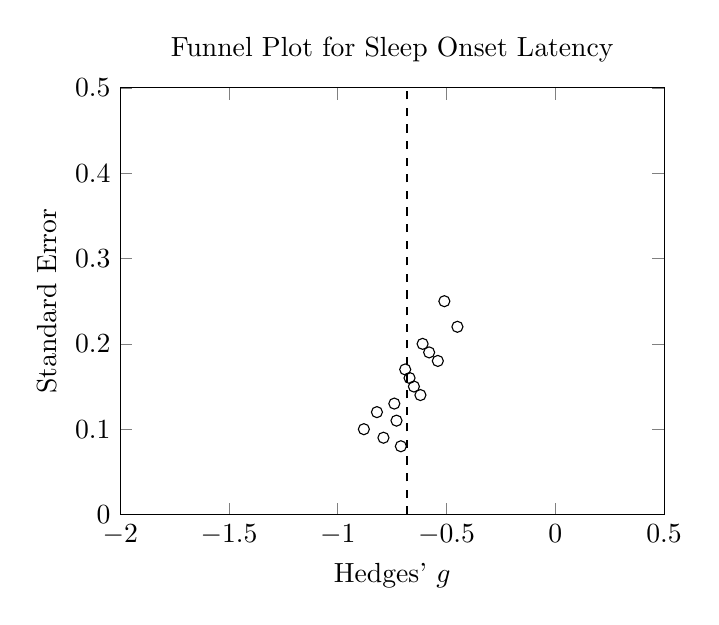
\begin{tikzpicture}
        \begin{axis}[
            xlabel={Hedges' $g$},
            ylabel={Standard Error},
            title={Funnel Plot for Sleep Onset Latency},
            width=0.7\textwidth,
            height=7cm,
            xmin=-2, xmax=0.5,
            ymin=0, ymax=0.5,
        ]
        % Placeholder points representing studies
        \addplot[only marks, mark=o] coordinates {
            (-0.82,0.12) (-0.65,0.15) (-0.54,0.18) (-0.71,0.08) (-0.45,0.22)
            (-0.88,0.10) (-0.62,0.14) (-0.73,0.11) (-0.58,0.19) (-0.67,0.16)
            (-0.79,0.09) (-0.51,0.25) (-0.74,0.13) (-0.61,0.20) (-0.69,0.17)
        };
        \draw[thick, dashed] (axis cs:-0.68,0) -- (axis cs:-0.68,0.5);
        \end{axis}
    \end{tikzpicture}
    \caption{Funnel plot of effect sizes for sleep onset latency. The dashed line
             represents the pooled estimate. Symmetry suggests minimal publication bias.}
    \label{fig:funnel}
\end{figure}

\subsection{Moderator Analyses}

Delivery format significantly moderated treatment efficacy for SOL ($Q_M = 8.42$,
$p = .015$). Individual delivery ($g = -0.78$) produced larger effects than group
delivery ($g = -0.54$) or digital delivery ($g = -0.49$). Treatment duration also
moderated effects, with $\geq$ 6-week interventions ($g = -0.74$) outperforming
shorter interventions ($g = -0.52$; $Q_M = 5.89$, $p = .015$).

\subsection{Publication Bias}

Egger's test was not significant for SOL ($p = .18$), WASO ($p = .24$), or TST
($p = .31$), suggesting no funnel plot asymmetry. Trim-and-fill analysis identified
one imputed study for SE, with the adjusted effect size remaining significant
($g_{\text{adj}} = 0.68$, 95\% CI $[0.54, 0.82]$).

\section{Discussion}
\label{sec:discussion}

This meta-analysis demonstrates that CBT-I is effective in older adults, with
moderate-to-large effect sizes across all primary outcomes. The effect size for sleep
efficiency ($g = 0.72$) is particularly noteworthy, as SE is a key target of CBT-I
and is strongly associated with subjective sleep quality.

Our moderator analyses suggest that individual delivery may be preferable for older
adults, possibly because it allows for greater personalization of sleep restriction
schedules and cognitive restructuring exercises. The finding that longer treatment
durations are more effective aligns with clinical recommendations for adapted CBT-I
in this population \cite{mack2019cognitive}.

\section{Limitations}
\label{sec:limitations}

Several limitations should be noted. First, the majority of included studies used
subjective sleep measures; future meta-analyses should focus on polysomnographic
outcomes when sufficient data are available. Second, heterogeneity was moderate to
high across outcomes, indicating variability in treatment effects that may be
attributable to unmeasured moderators. Third, most studies were conducted in Western
countries, limiting generalizability.

\section{Conclusions}
\label{sec:conclusions}

CBT-I is an evidence-based treatment for insomnia in older adults. Healthcare
providers should prioritize CBT-I over pharmacotherapy as the first-line treatment.
Future research should investigate mechanisms of change, optimal delivery formats,
and long-term maintenance of treatment gains.

\bibliographystyle{apa}
\bibliography{references}

\end{document}
